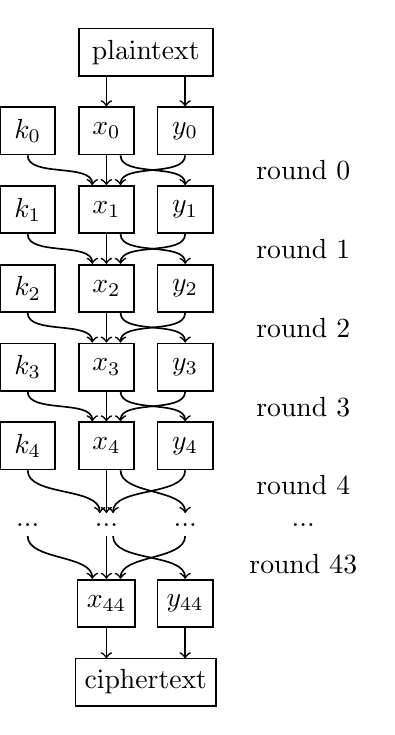
\begin{tikzpicture}
	[line width=0.6,trim left,
	box/.style = {
		draw,
		minimum height = 0.6cm,
		minimum width = 0.7cm
	},
	bigbox/.style = {
		draw,
		minimum height = 0.6cm,
		minimum width = 1.7cm
	},
	keybox/.style = {
		draw,
		minimum height = 3.6cm,
		minimum width = 0.7cm
	},
	nobox/.style = {
		minimum width = 0.7cm
	},
	wire/.style = {
		looseness=0.8,
		out=270,
		in=90
	},
	xor/.style = {
		draw, circle, inner sep=0cm, minimum size=0.4cm,
		append after command = {
			[shorten >=\pgflinewidth, shorten <=\pgflinewidth,]
			(\tikzlastnode.north) edge (\tikzlastnode.south)
			(\tikzlastnode.east) edge (\tikzlastnode.west)
		}
	},
	odot/.style = {
		draw, circle, inner sep=0cm, minimum size=0.4cm
	},
	dot/.style = {
		fill, circle, inner sep=0cm, minimum size=0.08cm
	},
	invisible/.style = {
		minimum size=0cm
	}]
	
	
	%Draw nodes
	\node[bigbox] at (1.5,7) (pt) {plaintext};
	\node[keybox] at (-1, 4.5) (key) {$K$};
	\node[box] at (1,6) (x0) {$x_0$};
	\node[box] at (2,6) (y0) {$y_0$};
	\node[box] at (0,6) (k0) {$k_0$};
	
	\node[box] at (1,5) (x1) {$x_1$};
	\node[box] at (2,5) (y1) {$y_1$};
	\node[box] at (0,5) (k1) {$k_1$};
	
	\node[box] at (1,4) (x2) {$x_2$};
	\node[box] at (2,4) (y2) {$y_2$};
	\node[box] at (0,4) (k2) {$k_2$};
	
	\node[box] at (1,3) (x3) {$x_3$};
	\node[box] at (2,3) (y3) {$y_3$};
	\node[box] at (0,3) (k3) {$k_3$};
	
	\node[box] at (1,2) (x4) {$x_4$};
	\node[box] at (2,2) (y4) {$y_4$};
	\node[box] at (0,2) (k4) {$k_4$};
	
	\node[nobox] at (1,1) (x5) {$...$};
	\node[nobox] at (2,1) (y5) {$...$};
	\node[nobox] at (0,1) (k5) {$...$};
	
	
	\node[box] at (1,0) (x44) {$x_{44}$};
	\node[box] at (2,0) (y44) {$y_{44}$};
	\node[bigbox] at (1.5,-1) (ct) {ciphertext};
	
	\coordinate(pt1) at (1,6.7);
	\coordinate(pt2) at (2,6.7);
	\coordinate(ct1) at (1,-0.7);
	\coordinate(ct2) at (2,-0.7);
	
	\coordinate(K0) at (-0.65,6);
	\coordinate(K1) at (-0.65,5);
	\coordinate(K2) at (-0.65,4);
	\coordinate(K3) at (-0.65,3);
	
	\node[nobox] at (3.5,5.5) {round 0};
	\node[nobox] at (3.5,4.5) {round 1};
	\node[nobox] at (3.5,3.5) {round 2};
	\node[nobox] at (3.5,2.5) {round 3};
	\node[nobox] at (3.5,1.5) {round 4};
	\node[nobox] at (3.5,1) {$...$};
	\node[nobox] at (3.5,0.5) {round 43};
	
	%Draw wires
	
	\draw[wire,->] (pt1) to (x0);
	\draw[wire,->] (pt2) to (y0);
	
	\draw[wire,->] (K0) to[out=0, in=180] (k0.180);
	\draw[wire,->] (K1) to[out=0, in=180] (k1.180);
	\draw[wire,->] (K2) to[out=0, in=180] (k2.180);
	\draw[wire,->] (K3) to[out=0, in=180] (k3.180);
	
	\draw[wire,->] (x0.300) to (y1.90);
	\draw[wire,->] (x0.270) to (x1.90);
	\draw[wire,->] (y0.270) to (x1.60);
	\draw[wire,->] (k0.270) to (x1.120);
	
	\draw[wire,->] (x1.300) to (y2.90);
	\draw[wire,->] (x1.270) to (x2.90);
	\draw[wire,->] (y1.270) to (x2.60);
	\draw[wire,->] (k1.270) to (x2.120);
	
	\draw[wire,->] (x2.300) to (y3.90);
	\draw[wire,->] (x2.270) to (x3.90);
	\draw[wire,->] (y2.270) to (x3.60);
	\draw[wire,->] (k2.270) to (x3.120);
	
	\draw[wire,->] (x3.300) to (y4.90);
	\draw[wire,->] (x3.270) to (x4.90);
	\draw[wire,->] (y3.270) to (x4.60);
	\draw[wire,->] (k3.270) to (x4.120);

	\draw[wire,->] (x4.300) to (y5.90);
	\draw[wire,->] (x4.270) to (x5.90);
	\draw[wire,->] (y4.270) to (x5.60);
	\draw[wire,->] (k4.270) to (x5.120);
	
	\draw[wire,->] (x5.300) to (y44.90);
	\draw[wire,->] (x5.270) to (x44.90);
	\draw[wire,->] (y5.270) to (x44.60);
	\draw[wire,->] (k5.270) to (x44.120);
	
	\draw[wire,->] (x44) to (ct1);
	\draw[wire,->] (y44) to (ct2);
	
\end{tikzpicture} 